%%%%%%%%%%%%%%%%%%%%%%%%%%%%%%%%%%%%%%%%%
% Structured General Purpose Assignment
% LaTeX Template
%
% This template has been downloaded from:
% http://www.latextemplates.com
%
% Original author:
% Ted Pavlic (http://www.tedpavlic.com)
%
% Note:
% The \lipsum[#] commands throughout this template generate dummy text
% to fill the template out. These commands should all be removed when 
% writing assignment content.
%
%%%%%%%%%%%%%%%%%%%%%%%%%%%%%%%%%%%%%%%%%


%----------------------------------------------------------------------------------------
%	PACKAGES AND OTHER DOCUMENT CONFIGURATIONS
%----------------------------------------------------------------------------------------

\documentclass{article}

%\usepackage{currfile}
\usepackage{fancyhdr} % Required for custom headers
\usepackage{lastpage} % Required to determine the last page for the footer
\usepackage{extramarks} % Required for headers and footers
\usepackage{graphicx} % Required to insert images
\usepackage{lipsum} % Used for inserting dummy 'Lorem ipsum' text into the template
\usepackage{outlines}
\usepackage{wrapfig}
\usepackage[dutch,]{babel}
\selectlanguage{dutch}

\usepackage{xcolor}
\usepackage{listings}	% om SQL code toe te voegen aan document

% Margins
\topmargin=-0.45in
\evensidemargin=0in
\oddsidemargin=0in
\textwidth=6.5in
\textheight=9.0in
\headsep=0.25in 

\linespread{1.1} % Line spacing

% Set up the header and footer
\pagestyle{fancy}
\lhead{\hmwkAuthorName} % Top left header
%\chead{\hmwkClass\ \small{(\textit{\hmwkClassInstructor})}} 
\chead{\hmwkClass} 
\rhead{\hmwkTitle} 
\lfoot{\LaTeX: \small{\input{filename.txt}}} % Bottom left footer
%\lfoot{\LaTeX: {/home/jan/CVOTSM/A7\_IT-organisatie/ITIL/}\currfilepath} % Bottom left footer
\cfoot{} % Bottom center footer
\rfoot{Pagina\ \thepage\ van\ \pageref{LastPage}} % Bottom right footer
\renewcommand\headrulewidth{0.4pt} % Size of the header rule
\renewcommand\footrulewidth{0.4pt} % Size of the footer rule

\setlength\parindent{0pt} % Removes all indentation from paragraphs


%\setlength{\parskip}{\baselineskip}%
%\setlength{\parindent}{12pt}%

%----------------------------------------------------------------------------------------
%	DOCUMENT STRUCTURE COMMANDS
%	Skip this unless you know what you're doing
%----------------------------------------------------------------------------------------

% Header and footer for when a page split occurs within a problem environment
\newcommand{\enterProblemHeader}[1]{
\nobreak\extramarks{#1}{#1 continued on next page\ldots}\nobreak
\nobreak\extramarks{#1 (continued)}{#1 continued on next page\ldots}\nobreak
}

% Header and footer for when a page split occurs between problem environments
\newcommand{\exitProblemHeader}[1]{
\nobreak\extramarks{#1 (continued)}{#1 continued on next page\ldots}\nobreak
\nobreak\extramarks{#1}{}\nobreak
}

\setcounter{secnumdepth}{0} % Removes default section numbers
\newcounter{homeworkProblemCounter} % Creates a counter to keep track of the number of problems

\newcommand{\homeworkProblemName}{}
\newenvironment{homeworkProblem}[1][Problem \arabic{homeworkProblemCounter}]{ % Makes a new environment called homeworkProblem which takes 1 argument (custom name) but the default is "Problem #"
\stepcounter{homeworkProblemCounter} % Increase counter for number of problems
\renewcommand{\homeworkProblemName}{#1} % Assign \homeworkProblemName the name of the problem
\section{\homeworkProblemName} % Make a section in the document with the custom problem count
\enterProblemHeader{\homeworkProblemName} % Header and footer within the environment
}{
\exitProblemHeader{\homeworkProblemName} % Header and footer after the environment
}

\newcommand{\problemAnswer}[1]{ % Defines the problem answer command with the content as the only argument
\noindent\framebox[\columnwidth][c]{\begin{minipage}{0.98\columnwidth}#1\end{minipage}} % Makes the box around the problem answer and puts the content inside
}

\newcommand{\homeworkSectionName}{}
\newenvironment{homeworkSection}[1]{ % New environment for sections within homework problems, takes 1 argument - the name of the section
\renewcommand{\homeworkSectionName}{#1} % Assign \homeworkSectionName to the name of the section from the environment argument
\subsection{\homeworkSectionName} % Make a subsection with the custom name of the subsection
\enterProblemHeader{\homeworkProblemName\ [\homeworkSectionName]} % Header and footer within the environment
}{
\enterProblemHeader{\homeworkProblemName} % Header and footer after the environment
}
   
%----------------------------------------------------------------------------------------
%	NAME AND CLASS SECTION
%----------------------------------------------------------------------------------------

\newcommand{\hmwkTitle}{5. Datawoordenboek} % Assignment title
%\newcommand{\hmwkDueDate}{Monday,\ January\ 1,\ 2012} % Due date
\newcommand{\hmwkDueDate}{} % Due date
\newcommand{\hmwkClass}{Projectwerk} % Course/class
%\newcommand{\hmwkClassTime}{10:30am} % Class/lecture time
\newcommand{\hmwkClassTime}{} % Class/lecture time
\newcommand{\hmwkClassInstructor}{} % Teacher/lecturer
\newcommand{\hmwkAuthorName}{Wagemakers Jan} % Your name

%----------------------------------------------------------------------------------------
%	TITLE PAGE
%----------------------------------------------------------------------------------------

\title{
\vspace{2in}
\textmd{\textbf{\hmwkClass}}\\
\textmd{\textbf{\hmwkTitle}}\\
%\normalsize\vspace{0.1in}\small{In\ te\ dienen\ voor\ \hmwkDueDate}\\
%\vspace{0.1in}{\textit{Leerkracht: \hmwkClassInstructor\ \hmwkClassTime}}
\vspace{3in}
}

\author{\textbf{\hmwkAuthorName}}
\date{\today} % Insert date here if you want it to appear below your name

%----------------------------------------------------------------------------------------

\begin{document}

\maketitle

%----------------------------------------------------------------------------------------
%	TABLE OF CONTENTS
%----------------------------------------------------------------------------------------

%\setcounter{tocdepth}{1} % Uncomment this line if you don't want subsections listed in the ToC

%\newpage
%\tableofcontents
\newpage

%%% Opdracht

%\begin{homeworkProblem}[\arabic{homeworkProblemCounter} : Omschrijving opdracht]
\begin{homeworkProblem}[Schematisch overzicht gegevens]
	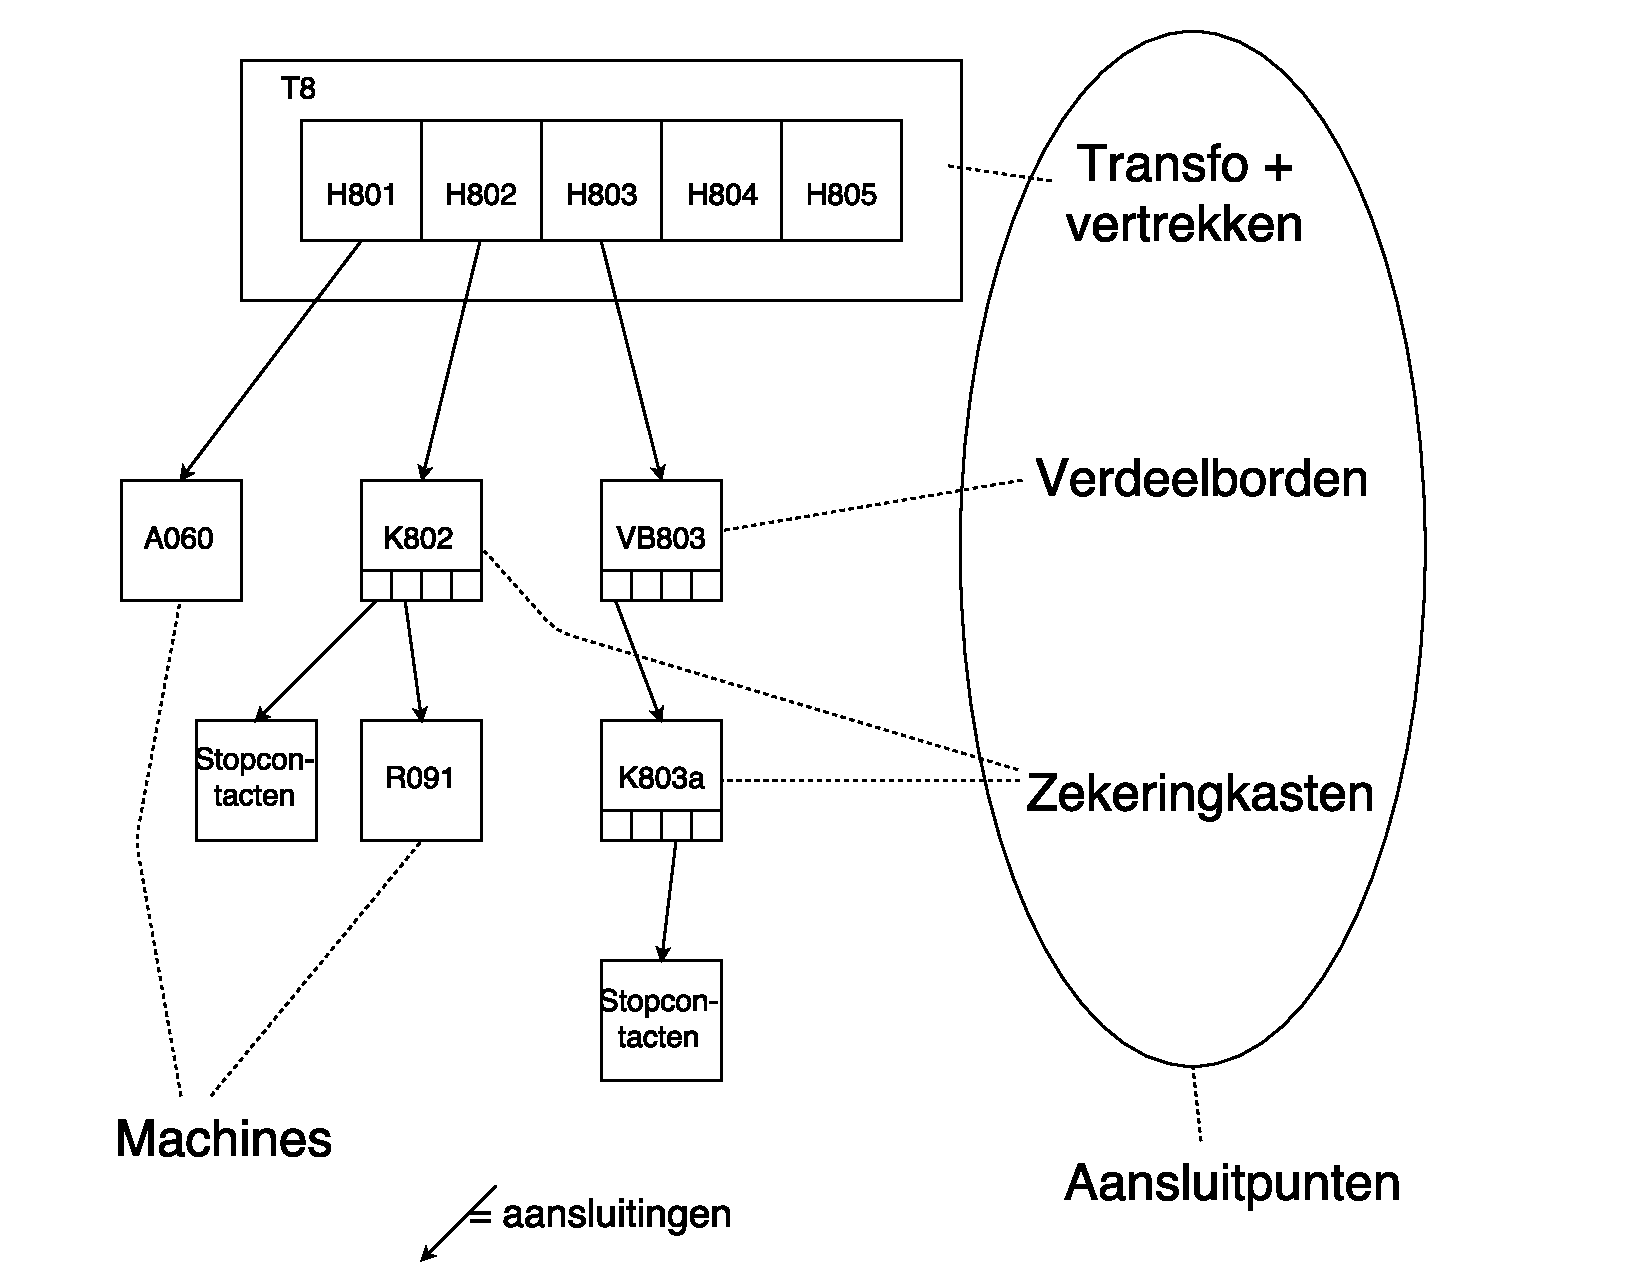
\includegraphics[width=1.2\textwidth]{pictures/Aansluitpunten.ps}
\end{homeworkProblem}
\newpage

\begin{homeworkProblem}[Aansluitpunten]
	\begin{center}
		\begin{tabular}{ | l | l | l | c | c | p{5cm} | }	\hline
			    Naam 				& Type    & Lengte & PRIMARY & NULL & Omschrijving \\ \hline
			    \texttt{\detokenize{AP_id}} 	& varchar & 10     & JA      & NEE  & Uniek ID van het aansluitpunt, bv.: T8, VB810, K810a \\ \hline
			    \texttt{\detokenize{AP_locatie}}	& varchar & 10	   & NEE     & JA   & Referentie plaats (grondplannummer) \\ \hline
		    \end{tabular}
	\end{center}
\end{homeworkProblem}

\begin{homeworkProblem}[Machines]
	\begin{center}
		\begin{tabular}{ | l | l | l | c | c | p{5cm} | }	\hline
			    Naam 					& Type    & Lengte & PRIMARY & NULL & Omschrijving \\ \hline
			    \texttt{\detokenize{M_id}} 			& varchar & 10     & JA      & NEE  & Uniek ID van de machine, bv. T029, R055, S019, I001 \\ \hline
			    \texttt{\detokenize{M_omschrijving}}	& varchar & 80     & NEE     & NEE  & Omschrijving van de machine \\ \hline
			    \texttt{\detokenize{M_locatie}}		& varchar & 10	   & NEE     & JA   & Referentie plaats (grondplannummer) \\ \hline
		    \end{tabular}
	\end{center}
\end{homeworkProblem}

\begin{homeworkProblem}[Aansluitingen]
	\begin{center}
		\begin{tabular}{ | l | l | l | c | c | p{5cm} | }	\hline
			    Naam 					& Type    	& Lengte & PRIMARY & NULL & Omschrijving \\ \hline
			    \texttt{\detokenize{A_id}}			& varchar 	& 10     & JA      & NEE  & Over welke aansluiting gaat het? bv. Sa, H810, Kring 3.1 \\ \hline
			    \texttt{\detokenize{AP_id}} 		& varchar 	& 10     & JA      & NEE  & Uniek ID van het aansluitpunt, bv.: T8, VB810, K810a \\ \hline
			    \texttt{\detokenize{Naar_AP_id}}		& varchar 	& 10 	 & NEE     & JA   & Naar welke aansluitpunt gaat deze aansluiting? Kan NULL zijn als deze aansluiting niet naar een ander aansluitpunt gaat \\ \hline
			    \texttt{\detokenize{Naar_M_id}}		& varchar 	& 10     & NEE     & JA   & Naar welke machine gaat deze aansluiting? Kan NULL zijn als deze aansluiting niet naar een machine gaat \\ \hline
			    \texttt{\detokenize{Omschrijving}}		& varchar 	& 80     & NEE     & JA   & Omschrijving van hetgene dat aangesloten is. Gebruiken als zowel APid en Mid == NULL, als Mid != NULL dan MOmschrijving gebruiken \\ \hline
			    \texttt{\detokenize{Kabeltype}}		& varchar 	& 7	 & NEE     & JA   & KabelType, bv. XVB \\ \hline
			    \texttt{\detokenize{Kabelsectie}}		& varchar 	& 12     & NEE     & JA   & KabelDoorMeter bv, 4G95 \\ \hline
			    \texttt{\detokenize{Stroom}} 		& smallINT 	& -	 & NEE     & JA   & Zekering in A \\ \hline
			    \texttt{\detokenize{Polen}} 		& tinyINT	& -	 & NEE	   & NEE  & Uit hoeveel polen bestaat deze aansluiting \\ \hline	
		    \end{tabular}
	\end{center}
\end{homeworkProblem}

\begin{homeworkProblem}[EER Diagram]
	\includegraphics[width=.95\textwidth]{pictures/EER.eps}
\end{homeworkProblem}

\begin{homeworkProblem}[SQL Script]
\lstset{ %
		language=SQL,
		morekeywords={tinyint},
           	showspaces=false,
           	basicstyle=\fontsize{8}{9}\ttfamily,
           	numbers=left,
           	numberstyle=\tiny,
           	commentstyle=\color{gray},
		breaklines=true,
%%  backgroundcolor=\color{white},   % choose the background color; you must add \usepackage{color} or \usepackage{xcolor}; should come as last argument
%%   basicstyle=\footnotesize,        % the size of the fonts that are used for the code
%%   breakatwhitespace=false,         % sets if automatic breaks should only happen at whitespace
%%   breaklines=true,                 % sets automatic line breaking
%%   captionpos=b,                    % sets the caption-position to bottom
%%   commentstyle=\color{mygreen},    % comment style
%%   deletekeywords={...},            % if you want to delete keywords from the given language
%%   escapeinside={\%*}{*)},          % if you want to add LaTeX within your code
%%   extendedchars=true,              % lets you use non-ASCII characters; for 8-bits encodings only, does not work with UTF-8
%   frame=single,	                   % adds a frame around the code
		columns=flexible,
   		keepspaces=true,                 % keeps spaces in text, useful for keeping indentation of code (possibly needs columns=flexible)
%%   keywordstyle=\color{blue},       % keyword style
%%   language=Octave,                 % the language of the code
%%   morekeywords={*,...},            % if you want to add more keywords to the set
%%   numbers=left,                    % where to put the line-numbers; possible values are (none, left, right)
%%   numbersep=5pt,                   % how far the line-numbers are from the code
%%   numberstyle=\tiny\color{gray}, % the style that is used for the line-numbers
%%   rulecolor=\color{black},         % if not set, the frame-color may be changed on line-breaks within not-black text (e.g. comments (green here))
%%   showspaces=false,                % show spaces everywhere adding particular underscores; it overrides 'showstringspaces'
%%   showstringspaces=false,          % underline spaces within strings only
%%   showtabs=false,                  % show tabs within strings adding particular underscores
%%   stepnumber=2,                    % the step between two line-numbers. If it's 1, each line will be numbered
%%   		stringstyle=\color{green},     % string literal style
   		tabsize=4,	                   % sets default tabsize to 2 spaces
%%		title=SQL-script                   % show the filename of files included with \lstinputlisting; also try caption instead of title
}

\lstinputlisting{/home/jan/MEGA/2017-2018/ProjectWerk/LaagSpanningsNet.sql}
\end{homeworkProblem}

\end{document}
